\begin{subsection}{Arrow commands}
When drawing simple graphs and other illustrations, the use of arrows is often essential.  There are two arrow commands in \MP{} for accommodating this need\Dash \texttt{drawarrow} and \texttt{drawdblarrow}.  Both of these commands require a path argument.  For example, \begin{center}\verb|drawarrow (0,0)--(72,72);|\end{center} draws an arrow beginning at \verb|(0,0)| and ending at \verb|(72,72)| along the line segment connecting these points.

The path argument of both \texttt{drawarrow} and \texttt{drawdblarrow} need not be line segmented paths\Dash they may be any \MP{} path.  The only difference between \texttt{drawarrow} and \texttt{drawdblarrow} is that \texttt{drawarrow} places an arrow head at the end of the path and \texttt{drawdblarrow} places an arrow head at the beginning and the end of the path.  As an example, to draw the curved path in Figure \ref{fig:draw1} with an arrow head at the end of the path (i.e., at \texttt{z3}), the following command can be used \begin{center}\verb|drawarrow z1{right}..z2{dir 45}..{up}z3;|\end{center} and is illustrated in Figure \ref{fig:draw2}.
\begin{figure}[ht]
	\begin{center}\textattachfile[color={0 0 0},mimetype={text/plain}]{draw_2.mp}{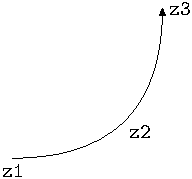
\includegraphics{draw_2}}\end{center}
	\caption{Using \texttt{drawarrow} along a path}\label{fig:draw2}
\end{figure}
\end{subsection}
